\section{Creearea unei aplicatii Android}
\subsection{Project template}
Sablonul pentru acest proiect poate fi descarcat de pe GitHub: \url{https://github.com/Dantsz/ProiectTWDM}
\subsubsection{Initializarea proiectului}
\begin{enumerate}
    \item clonati proiectul de pe GitHub
          \begin{lstlisting}
            git clone git@github.com:Dantsz/ProiectTWDM.git
        \end{lstlisting}
    \item deschideti Android Studio
    \item selectati \textit{Open}
    \item selectati directorul in care ati clonat proiectul
          \begin{figure}[H]
              \centering
              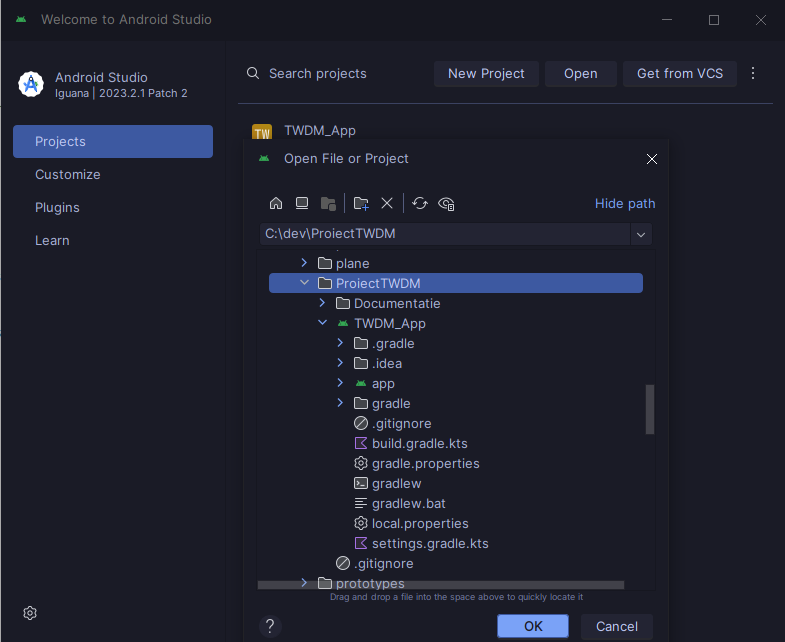
\includegraphics[width=0.7\linewidth]{figs/open_project.png}
              \caption{Deschiderea proiectului}
              \label{fig:open_project}
          \end{figure}
\end{enumerate}
\subsubsection{Structura proiectului}
\paragraph{Android Component Architecture}
\subsection{Rulare}